\documentclass[10pt,a4paper]{article}

\usepackage[margin=16mm]{geometry}
\usepackage[T1]{fontenc}
\usepackage[utf8]{inputenc}
\usepackage{lmodern}
\usepackage{microtype}
\usepackage{amsmath,amssymb}
\usepackage{booktabs}
\usepackage{enumitem}
\usepackage{xcolor}
\usepackage{tikz}
\usetikzlibrary{arrows.meta,positioning,fit}
\usepackage[colorlinks=true,linkcolor=black,urlcolor=blue!55!black,citecolor=black]{hyperref}
\usepackage{parskip}
\usepackage{titlesec}

\definecolor{ink}{HTML}{17202A}
\definecolor{muted}{HTML}{5D6D7E}
\definecolor{accent}{HTML}{185FA5}
\definecolor{pale}{HTML}{EEF5FB}
\definecolor{warn}{HTML}{FFF7E6}
\definecolor{line}{HTML}{CCD6E0}

\color{ink}
\setlength{\parindent}{0pt}
\setlength{\parskip}{4.5pt}
\setlist[itemize]{leftmargin=4.5mm,itemsep=1.5pt,topsep=2pt}
\setlist[enumerate]{leftmargin=5.5mm,itemsep=2pt,topsep=2pt}
\titleformat{\section}{\large\bfseries\color{accent}}{}{0pt}{}
\titlespacing*{\section}{0pt}{8pt}{3pt}
\titleformat{\subsection}{\normalsize\bfseries}{}{0pt}{}
\titlespacing*{\subsection}{0pt}{6pt}{2pt}

\newcommand{\callout}[2]{%
  \noindent\fcolorbox{line}{#1}{%
    \begin{minipage}{0.955\linewidth}
      #2
    \end{minipage}}
}

\begin{document}
\pagestyle{empty}

{\small\bfseries\color{accent} JAM RESEARCHER BRIEF}\par
\vspace{2pt}
{\LARGE\bfseries Does JAM maintain its capacity to correct shared implementation faults?}\par
\vspace{4pt}
{\small\color{muted} A narrow question for expert review of the JAM/ELVES security model. The aim is not to propose a replacement protocol model, but to test whether a residual failure mode has been identified or whether JAM already closes it elsewhere.}\par
\vspace{5pt}
\hrule

\section{The question}

Fix one invalid report and one fault family $x$. Some validators may be adversarial. A second group may be honest in the ordinary sense but share an implementation fault that makes this particular invalid report look valid. A third group independently detects the fault.

\callout{pale}{\textbf{Core distinction.} Validator honesty and implementation independence are different security resources. A validator can be honest yet fail to provide independent corrective capacity for a particular fault family.}

Let $A$ be adversarial validators, $B_x$ otherwise-honest validators sharing fault $x$, and $C_x$ validators that independently judge the report invalid, with $N=A+B_x+C_x$.

At the Gray-Paper verdict layer, the relevant arithmetic can be stated directly: if $K=\lfloor 2N/3\rfloor+1$, then independently correct negative judgments can construct a bad verdict against adversarial positive voting exactly when $C_x\ge K$ in the declared fault partition.

For the ELVES-style escalation model, let $F$ be the tranche/escalation factor, $\gamma=A/N$, and $f_x=B_x/(N-A)$. Replacing the generic honest share by the fault-specific independently correct share gives the declared reproduction mean
\[
\boxed{\lambda_x=F\frac{C_x}{N}=F(1-\gamma)(1-f_x),\qquad \lambda_x>1\ \text{supercritical}.}
\]
This substitution is a model extension, not a theorem attributed to the original ELVES analysis.

\subsection{A minimal counterexample}

Take the same validator count, the same adversarial share $\gamma=0.20$, and the same illustrative escalation factor $F=2$.

\begin{center}
\small
\begin{tabular}{@{}lccc@{}}
\toprule
 & shared-fault share $f_x$ & independently correct share & $\lambda_x$ \\
\midrule
Population 1 & $0.10$ & $0.80\times0.90=0.72$ & $1.44$ \\
Population 2 & $0.50$ & $0.80\times0.50=0.40$ & $0.80$ \\
\bottomrule
\end{tabular}
\end{center}

Both populations are 80\% non-adversarial. Under this declared audit model, one is above the independent-correction threshold and the other below it. Ordinary validator counts and honest fractions therefore do not determine fault-specific corrective capacity.

\begin{center}
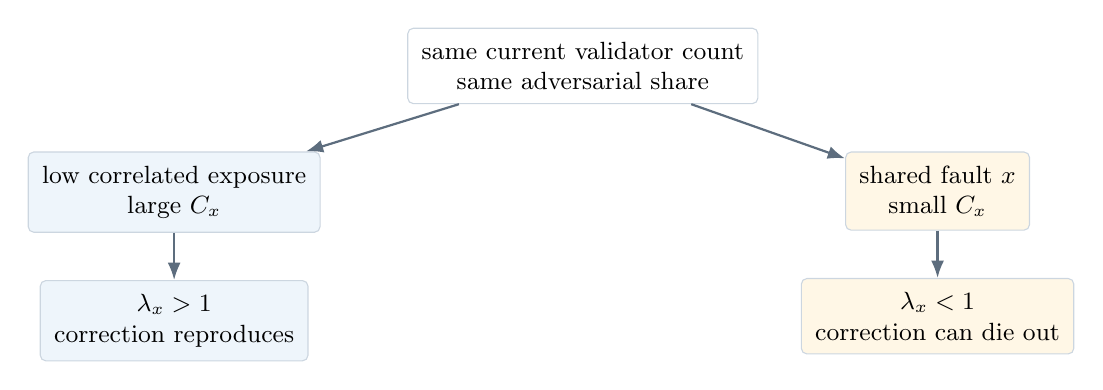
\begin{tikzpicture}[
  node distance=6mm and 11mm,
  box/.style={draw=line,rounded corners=2pt,fill=white,inner sep=5pt,align=center,font=\small},
  good/.style={box,fill=pale},
  bad/.style={box,fill=warn},
  arr/.style={-{Latex[length=2.2mm]},draw=muted,thick}
]
\node[box] (same) {same current validator count\\same adversarial share};
\node[good,below left=of same] (ind) {low correlated exposure\\large $C_x$};
\node[bad,below right=of same] (corr) {shared fault $x$\\small $C_x$};
\node[good,below=of ind] (sup) {$\lambda_x>1$\\correction reproduces};
\node[bad,below=of corr] (sub) {$\lambda_x<1$\\correction can die out};
\draw[arr] (same) -- (ind);
\draw[arr] (same) -- (corr);
\draw[arr] (ind) -- (sup);
\draw[arr] (corr) -- (sub);
\end{tikzpicture}
\end{center}

\section{The second question: what maintains correction over time?}

Even if $\lambda_x>1$ today, the ecosystem can lose the independent implementations, operators, effort, observability, or resources that supplied that margin. We therefore introduced the smallest explicit slow-state model we could use to separate \emph{current correction} from \emph{maintenance of future correction}.

Let $C_t$ denote normalized independently corrective capacity, $O_t$ maintenance observability/attribution, and $R_t$ returned-resource capacity. The declared slow loop is $C\rightarrow O\rightarrow R\rightarrow C$. Coupling the next slow update back to the audit layer gives
\[
\boxed{\lambda_{x,t+1}=r_C\lambda_{x,t}+F k_{RC}R_t.}
\]
At current criticality, $\lambda_{x,t}=1$, Lean verifies the exact one-step boundary
\[
\boxed{\lambda_{x,t+1}\ge1\quad\Longleftrightarrow\quad Fk_{RC}R_t\ge1-r_C.}
\]
Interpretation: return into corrective capacity must at least replace its attrition if a critical system is not to cross below the threshold on the next slow update.

\newpage

{\small\bfseries\color{accent} JAM RESEARCHER BRIEF \hfill PAGE 2}\par
\vspace{3pt}\hrule

\section{Why a snapshot is not enough}

The distinction does not depend on accepting the full three-variable maintenance model. In the reduced path $\lambda_t=m^t\lambda_0$, two systems can start at the same current value $\lambda_0=3/2$ but have opposite five-step status: with $m=1$ the value remains $3/2$; with $m=0.9$ it falls to approximately $0.886$.

\callout{pale}{\centering\textbf{Present agreement $\neq$ present corrective capacity $\neq$ maintained corrective capacity $\neq$ future corrective resilience.}}

The full-state Lean result goes one step further. For the declared $C\rightarrow O\rightarrow R\rightarrow C$ dynamics, it identifies a canonical replacement condition and proves a coordinatewise forward-invariant region in which fast audit correction stays supercritical at every future cross-audit time. It also proves the complementary erosion mechanism: remove the immediate $R\rightarrow C$ return edge while $r_C<1$, and positive corrective capacity declines at the next slow update.

\section{What is proved, and what is not claimed}

\begin{minipage}[t]{0.48\linewidth}
\textbf{Machine-checked in Lean}
\begin{itemize}
  \item separation of current audit correction from slow maintenance viability;
  \item witnesses for all four cells of the two-threshold phase structure;
  \item the one-step bridge from slow state to next-audit reproduction;
  \item eventual erosion in the reduced model when $0\le m<1$;
  \item the full-state forward-invariance persistence theorem;
  \item decline after deleting the immediate resource-return edge.
\end{itemize}
\end{minipage}\hfill
\begin{minipage}[t]{0.48\linewidth}
\textbf{Deliberately not claimed}
\begin{itemize}
  \item that $C_t,O_t,R_t$ are Gray-Paper state variables;
  \item that the coefficients are calibrated JAM quantities;
  \item that positive-systems, branching, or geometric-decay mathematics is novel;
  \item that the full slow system globally converges;
  \item that current JAM deployments have any particular correlated-fault rate.
\end{itemize}
\end{minipage}

\section{Three questions for JAM/ELVES reviewers}

\begin{enumerate}
\item \textbf{Coverage.} Is correlated honest implementation failure already covered by a JAM/ELVES assumption, verdict rule, sampling mechanism, or recovery mechanism that this analysis has missed?
\item \textbf{Security object.} If not, is \emph{fault-specific independently corrective capacity} a meaningful quantity for reasoning about JAM execution auditing, or is there a better protocol-native object?
\item \textbf{Measurement.} If the distinction is meaningful, which observable testnet/deployment quantities would best estimate whether independent corrective capacity persists across audits---client/fault-family exposure, independent re-execution effort, operator diversity, attribution, resource flows, or something else?
\end{enumerate}

\callout{warn}{\textbf{The requested expert judgment is intentionally narrow:} are we modelling a real residual failure mode of JAM, or has the protocol already closed this loop somewhere we have missed? If the latter, identifying that mechanism would directly falsify or substantially narrow the JAM-specific interpretation.}

\section{Where to inspect the full argument}

The full derivation, claim ledger, Python experiments, and machine-checked Lean proofs are collected in \href{https://github.com/albertjanvanhoek/Distributed-Commons-Control/pull/22}{Distributed-Commons-Control, PR \#22}. The most relevant source paths are:
\begin{itemize}
  \item \texttt{papers/correlated-honest-failure/} --- manuscript and claim ledger;
  \item \texttt{formalization/JamRecurrentMaintenance.lean};
  \item \texttt{formalization/JamResilienceDynamics.lean};
  \item \texttt{formalization/JamMaintenancePersistence.lean}.
\end{itemize}

\vfill
{\footnotesize\color{muted} Researcher brief, September 2026. This document is an interface to the formal work, not an additional layer of claims. The declared model is intentionally small so that protocol experts can reject, replace, or operationalize its assumptions.}

\end{document}
